\subsubsection{Activity Diagram - Module Biểu mẫu}

    Để minh họa chi tiết luồng xử lý của các chức năng chính trong module Biểu mẫu, báo cáo trình bày 2 Activity Diagram đại diện cho các pattern quan trọng trong hệ thống:
    
    \begin{itemize}
        \item \textbf{Template parsing \& configuration:} Tải lên và phân tích file Word template, trích xuất placeholder động, cấu hình trường dữ liệu (UC8.1)
        \item \textbf{Dynamic form generation:} Sinh form động từ cấu hình, điền dữ liệu, thay thế placeholder và tạo file Word/PDF tự động (UC8.2)
    \end{itemize}

    Mỗi diagram thể hiện luồng xử lý hoàn chỉnh từ đầu vào của người dùng đến kết quả cuối cùng, bao gồm các điểm phân nhánh (decision point) và xử lý ngoại lệ quan trọng.

    % ========================================
    % Activity Diagram UC8.1 - Tạo và cấu hình biểu mẫu
    \newpage
    \begin{figure}[H]
        \centering
        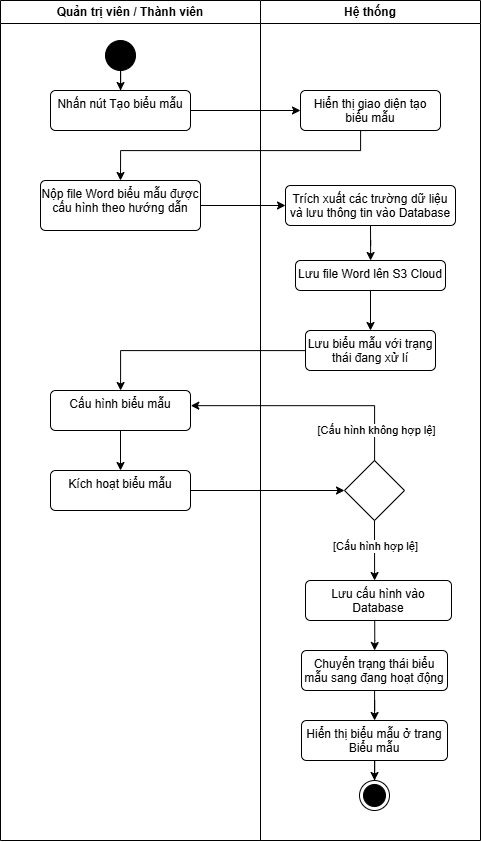
\includegraphics[width=0.75\linewidth]{Images/activity-diagram/UC08_01_tao_cau_hinh_bieu_mau.png}
        \vspace{0.3em}
        \captionsetup{skip=8pt}
        \caption{Activity Diagram - Tạo và cấu hình biểu mẫu}
        \label{fig:activity-uc08-01}
    \end{figure}

    Activity Diagram trên minh họa luồng tải lên và cấu hình biểu mẫu Word động. Hệ thống nhận file .docx, parse nội dung và trích xuất các placeholder theo cú pháp \{\{tên\_trường\}\}. Nếu không tìm thấy placeholder nào, hệ thống vẫn cho phép lưu template (có thể là biểu mẫu tĩnh) nhưng hiển thị cảnh báo. Sau khi trích xuất thành công, người dùng cấu hình cho từng placeholder: loại dữ liệu (text, number, date), nhãn hiển thị, và trường bắt buộc/tùy chọn. File template được lưu trên S3 Cloud và cấu hình trường được lưu vào database để sử dụng khi sinh form.

    % ========================================
    % Activity Diagram UC8.2 - Điền biểu mẫu
    \newpage
    \begin{figure}[H]
        \centering
        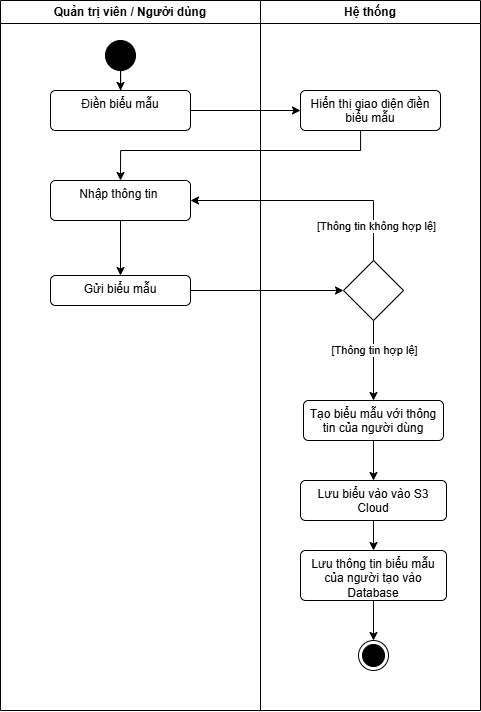
\includegraphics[width=0.75\linewidth]{Images/activity-diagram/UC08_02_dien_bieu_mau.png}
        \vspace{0.3em}
        \captionsetup{skip=8pt}
        \caption{Activity Diagram - Điền thông tin vào biểu mẫu}
        \label{fig:activity-uc08-02}
    \end{figure}

    Activity Diagram thể hiện luồng điền biểu mẫu động và sinh file tự động. Hệ thống lấy cấu hình trường từ database để sinh form với các input phù hợp (text box, number input, date picker). Sau khi người dùng điền thông tin, hệ thống validate theo cấu hình (kiểm tra trường bắt buộc, định dạng dữ liệu). Nếu hợp lệ, hệ thống tải template từ S3, thay thế các placeholder bằng dữ liệu người dùng nhập, và sinh file Word/PDF mới. File được lưu lại trên S3 để người dùng có thể tải xuống hoặc xem trước trong browser. Toàn bộ quá trình được lưu thành bản ghi nộp (submission) trong database để tra cứu sau này.
